\documentclass{../paper}

\begin{document}

\title{Diode Laser Absorption Spectroscopy \\ {\em Post-lab}}

\author{Iago B.~Mendes\,\orcidlink{0009-0007-9845-8448}}
\email{ibrazmen@oberlin.edu}
\affiliation{Department of Physics and Astronomy, Oberlin College, Oberlin, Ohio 44074, USA}

\date{\today}

\maketitle

\section{Background}

For both rubidium-85 ($^{85}$Rb) and rubidium-87 ($^{87}$Rb), the outermost electron's ground state is in the 5s orbital. The next excited state is in the 5p orbital. Figure \ref{fig:splittings} shows how both of these states get branches by fine and hyperfine splittings.

The fine splitting occurs due to a spin-orbit interaction. This happens because the electron's spin interacts with the magnetic field produced by its motion around the nucleus. The strength of this interaction depends on the electron's orbital angular momentum. Since the 5s orbital has no orbital angular momentum ($\ell = 0$) and the 5p orbital has some orbital angular momentum ($\ell = 1$), the fine splitting occurs only in the excited state. This is where we define two kinds of excitations: $D_1$ transition (going from the ground state to the lower excited state) and $D_2$ transition (going from the ground state to the higher excited state).

The hyperfine splitting occurs due to an electron-nucleus interaction. The nucleus has its own magnetic moment, which interacts with the magnetic field created by the electron. This effect is much smaller than fine splitting, but it still causes each energy level to split further. The hyperfine splitting affects all the prior energy levels (1 for the ground state and 2 for the excited state). In Figure \ref{fig:splittings}, the hyperfine splittings for the excited states were intentionally made much smaller than the hyperfine splittings for the ground state. In this experiment, it turns out that we do not have enough resolution to resolve the hyperfine splittings of the excited states. Therefore, we focus only on the hyperfine splitting of the ground state $\Delta\nu$. Since the $D_1$ and $D_2$ transitions start from the same ground-state level, both of them can be used to determine $\Delta\nu$. Here, we choose to use the $D_2$ transition for the reasons outlined in \cite{Brandenberger}.

\begin{figure*}
  \centering
  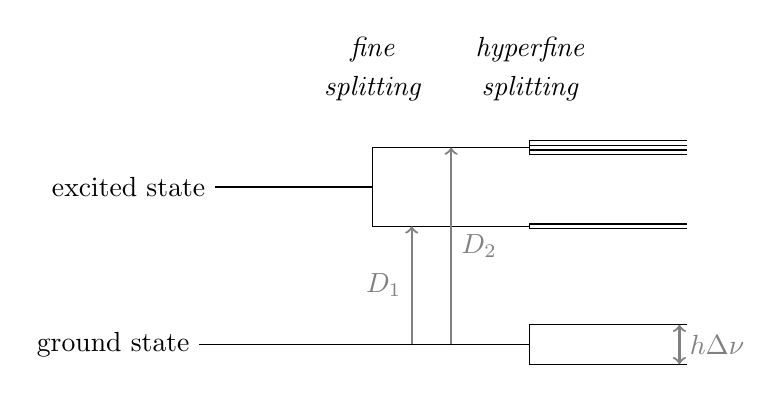
\begin{tikzpicture}
    \draw (-0.2,0) node[anchor = east] {ground state} -- (4,0);
    \draw (4,0) -- (4,0.25) -- (6,0.25);
    \draw (4,0) -- (4,-0.25) -- (6,-0.25);

    \node at (2,3.75) {\em fine};
    \node at (2,3.25) {\em splitting};
    \node at (4,3.75) {\em hyperfine};
    \node at (4,3.25) {\em splitting};

    \draw (0,2) node[anchor = east] {excited state} -- (2,2);
    \draw (2,2) -- (2,2.5) -- (4,2.5);
    \draw (2,2) -- (2,1.5) -- (4,1.5);
    \draw (4,2.5) -- (4,2.59) -- (6,2.59);
    \draw (4,2.5) -- (4,2.53) -- (6,2.53);
    \draw (4,2.5) -- (4,2.47) -- (6,2.47);
    \draw (4,2.5) -- (4,2.41) -- (6,2.41);
    \draw (4,1.5) -- (4,1.53) -- (6,1.53);
    \draw (4,1.5) -- (4,1.47) -- (6,1.47);

    \draw[->, thick, color=gray] (2.5,0) -- (2.5,1.5) node[pos = 0.5, anchor = east] {$D_1$};
    \draw[->, thick, color=gray] (3,0) -- (3,2.5) node[pos = 0.5, anchor = west] {$D_2$};

    \draw[<->, thick, color=gray] (5.9,-0.25) -- (5.9,0.25) node[pos = 0.5, anchor = west] {$h \Delta \nu$};
  \end{tikzpicture}

  \caption{Energy diagram with fine and hyperfine splittings.}
  \label{fig:splittings}
\end{figure*}

\section{Procedure}

We used a semiconductor laser diode for this experiment to generate a tunable laser beam. The wavelength of the emitted light can be adjusted by changing the injected laser current. As the current increases, the population of electrons and holes in the conduction and valence bands also increases, which leads to more electron-hole recombination, enhancing the stimulated emission and shifting the wavelength \cite{Svelto}. Additionally, as the temperature of the semiconductor laser diode increases, the bandgap energy of the semiconductor typically decreases, shifting the wavelength \cite{Svelto}.

To control the frequency of the laser, we use a Fabry-Perot resonator, which transmits only certain frequencies. This allows us to identify discrete transmission peaks that correspond to specific frequency gaps emitted by the laser diode. The ability to convert time to frequency is limited by the resolution of the Fabry-Perot interferometer, which is determined by the separation between the Fabry-Perot mirrors.

\section{Results}

We recorded both the transmission and absorption data as functions of time $t$, as shown in Figure \ref{fig:time_plot}. We manually selected the times for each peak and used Igor Pro to find a fit function as
\begin{equation}
  N(t) = K_0 + K_1 t + K_2 t^2 + K_3 t^3,
\end{equation}
where $N(t)$ is the number of peaks at a given time $t$. The fit coefficients given by Igor Pro were
\begin{align}
  K_0 &= -0.6(2), \\
  K_1 &= 1910(50), \\
  K_2 &= 60000(4000), \\
  K_3 &= -1.57(8) \times 10^6.
\end{align}
To get a time-to-frequency conversion, we need to know the free spectral range of our Fabry-Perot resonator. We measured its length to be
\begin{equation}
  L = 900(1) \text{ mm},
\end{equation}
which gives us a free spectral range of
\begin{equation}
  \Delta \nu_\text{FSR} = \frac{c}{2 n L} = 166.6(2) \text{ MHz}.
\end{equation}
Since the frequency spacing between transmission peaks is uniform, we know that
\begin{equation}
  \nu(N) = \Delta \nu_\text{FSR} N + \nu_0,
\end{equation}
where $\nu_0$ is some offset. Then, our conversion function is
\begin{align}
  \nu(t)
  &= \Delta \nu_\text{FSR} N(t) + \nu_0 \\
  &= \Delta \nu_\text{FSR} (K_0 + K_1 t + K_2 t^2 + K_3 t^3) + \nu_0.
\end{align}

Applying this conversion function to our absorption data, we have the result shown in Figure \ref{fig:analysis}, where we also show the Gaussian fits done to identify the four absorption peaks. By comparing with the literature values in \cite{RbData}, we find that the first and fourth peaks correspond to $^{87}$Rb, for which we find a hyperfine splitting of
\begin{equation}
  \Delta\nu(^{87}\text{Rb}) = 6.5(5) \text{ GHz}.
\end{equation}
Similarly, we find that the second and third peaks correspond to $^{85}$Rb, for which we find a hyperfine splitting of
\begin{equation}
  \Delta\nu(^{85}\text{Rb}) = 2.9(3) \text{ GHz}.
\end{equation}

Using the standard deviation of our Gaussian fits, we can compute the full-width at half-maximum (FWHM) of our resonance curves. Doing so, we get
\begin{align}
  \Delta\nu_1 &= 516 \text{ MHz}, \\
  \Delta\nu_2 &= 591 \text{ MHz}, \\
  \Delta\nu_3 &= 571 \text{ MHz}, \\
  \Delta\nu_4 &= 488 \text{ MHz}.
\end{align}
According to \cite{Brandenberger}, we expect that our laser wavelength (near 780 nm) would suffer from Doppler broading with a FWHM of 502 MHz. Evidently, there is a lot of variation in our reported widths, which are likely due to the misalignment of the base of the absorption peaks. In another iteration of this experiment, it would be ideal to vary the laser parameters to address this issue.

\begin{figure*}
  \centering
  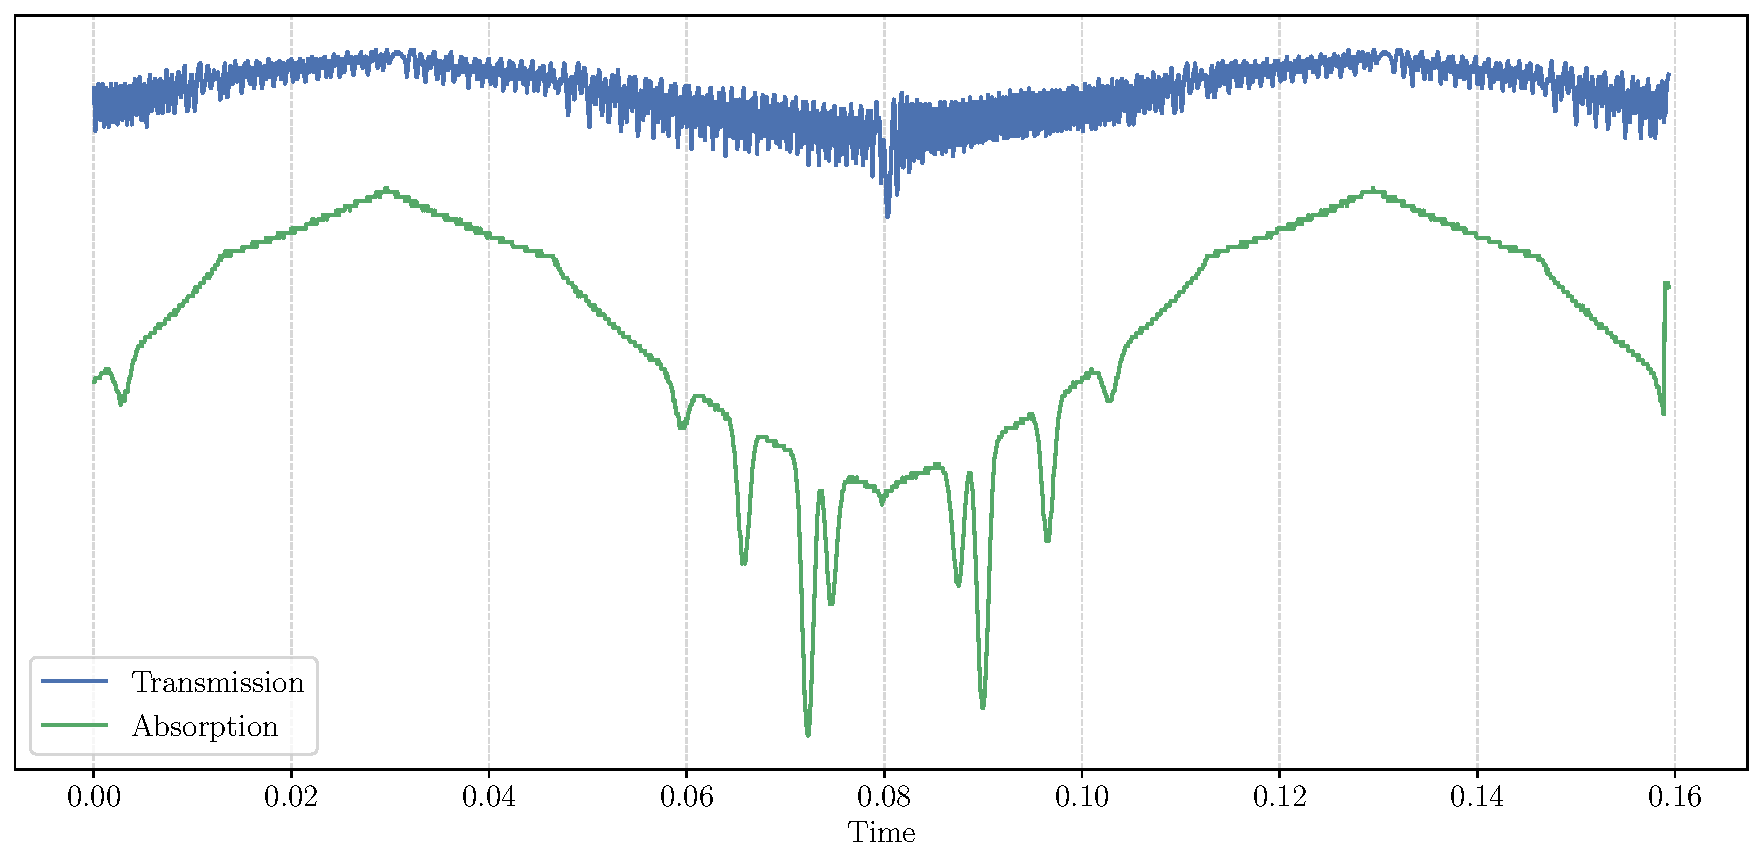
\includegraphics[width=0.8\textwidth]{data/time_plot.pdf}
  \caption{Transmission and absorption data as a function of sweep time.}
  \label{fig:time_plot}
\end{figure*}

\begin{figure*}
  \centering
  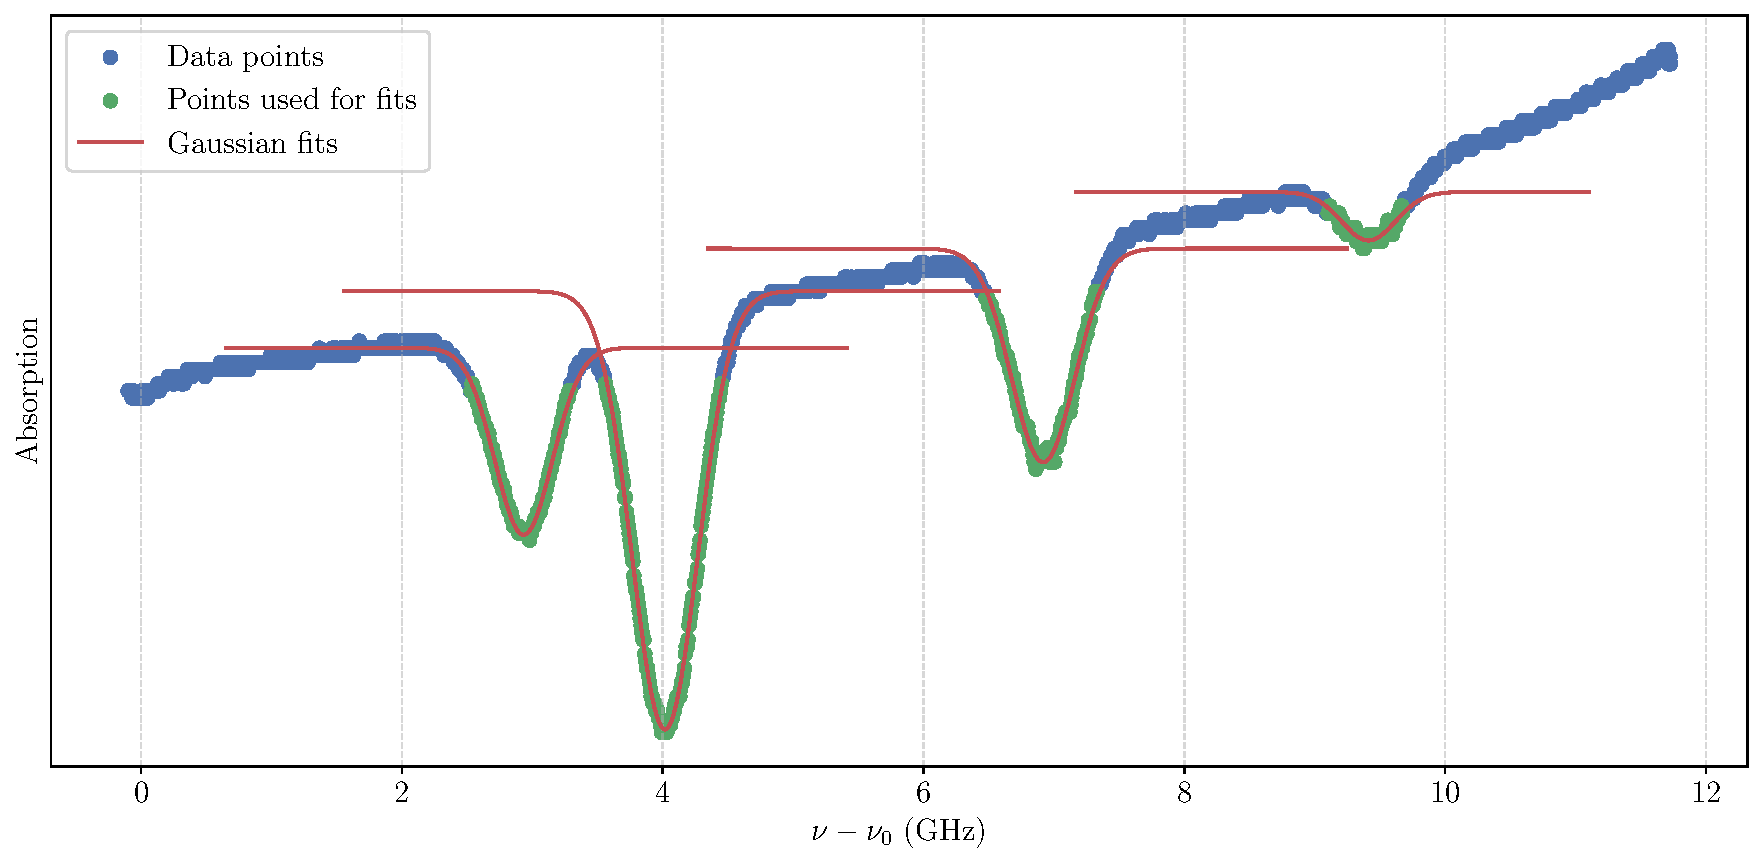
\includegraphics[width=0.8\textwidth]{data/analysis.pdf}
  \caption{Absorption data as a function of frequency.}
  \label{fig:analysis}
\end{figure*}

\begin{acknowledgements}
  This work was done in collaboration with Avay Subedi under the supervision of Professor Yuri Ijiri.
\end{acknowledgements}

\bibliography{refs}

\end{document}
